\documentclass[10pt]{beamer}
\usepackage{pgf}
\usepackage{colortbl,tabularx,amsfonts,mathrsfs,calligra}
\usepackage{ragged2e}
\usepackage{setspace}
\usepackage{tikz}
\usepackage{filecontents}
\usepackage{amsmath,amssymb}
\usepackage{tabularx}
\usepackage{xcolor}
\usepackage{xcolor}
\usepackage{physics}
\usepackage{esint}

\bibliographystyle{apalike}

\usetheme{CambridgeUS}
\usecolortheme{orchid}
\usefonttheme{professionalfonts}
\setbeamertemplate{theorems}[numbered]
\setbeamertemplate{bibliography item}{\insertbiblabel}
\setbeamercovered{transparent}

\setbeamercolor{highlighted}{fg=yellow,bg=black!50!blue!90}
\setbeamercolor{dimmed}{fg=white,bg=gray!50}
\setbeamercolor{boxbiru}{fg=yellow,bg=black!50!blue!90}
\setbeamercolor{boxpurple}{fg=white,bg=purple}
\setbeamercolor{boxpink}{fg=black,bg=pink}
\setbeamercolor{boxviolet}{fg=white,bg=violet}
\setbeamercolor{boxabu}{fg=black!30!blue!100,bg=gray!40}
\setbeamertemplate{background canvas}[vertical shading][bottom=red!15,top=blue!15]

\usetikzlibrary{shapes.geometric, arrows}

\newtheorem{theorems}{Teorema}
\newtheorem{Lemmas}[theorems]{Lema}
\newtheorem{remark}[theorems]{Catatan}
\newtheorem{proposition}[theorems]{Proposisi}
\newtheorem{algorithm}[theorems]{Algoritma}
\newtheorem{problems}[theorems]{Problem}
\newtheorem{exercise}[theorem]{Latihan}
\newtheorem{contoh}[theorems]{Contoh}
\newtheorem{corollaries}[theorems]{Akibat}
\newtheorem{definisi}{Definisi}

%\newproof{proof}{Proof}
\newenvironment{proofs}
{\paragraph{Proof:}}
{\hfill$\blacksquare$\newline}


 \pgfdeclareimage[height=.85cm]{logo}{logoITS}
 \logo{\pgfuseimage{logo}}


\title{ANALISIS VEKTOR RANGKUMAN BUKU SCHAUM}
\author{Kelompok 10\part{The Probability Theory}}
\institute{by Renaldy,Nicholas,Teo,Rico}
\date{JUNI 2024}

\newcommand{\kiri}{\left}
\newcommand{\kanan}{\right}

\begin{document}
\begin{frame}[plain]
    %\frametitle{\bf Analisis Real I}
    \transboxout
    \begin{beamercolorbox}[wd=\textwidth,rounded=true,shadow=true]{boxbiru}
        \centering
        \resizebox{.8\textwidth}{1em}{%
        \textsf{\textbf{RANGKUMAN BUKU SCHAUM}}}\\[1.5ex]
    \end{beamercolorbox}
    
    \vspace*{2ex}
    
        \transboxout
    \begin{beamercolorbox}[wd=\textwidth,rounded=true,shadow=true]{boxbiru}
        \centering
        \resizebox{.5\textwidth}{1em}{%
        \textsf{\textbf{DIBUAT OLEH : KELOMPOK 10}}}\\[0.5ex]
        
    \end{beamercolorbox}
    
%    \centerline{Bagian I}
%	\centerline{Himpunan dan Fungsi}

    \vspace*{6ex}

    \centerline{
\includegraphics[scale=.1]{logoITS}}

    \vspace*{2ex}

    \begin{center}
    \tiny
    \rm
    \color{magenta!50!cyan!100}
    INSTITUT TEKNOLOGI SEPULUH NOPEMBER\\
    Departemen Matematika\\
    %Institut Teknologi Sepuluh Nopember\\
    Indonesia\\
    \end{center}
\end{frame}%--------------------------------------------

\section{Daftar Anggota Kelompok}

{
    \begin{frame}
        \frametitle{Daftar Anggota Kelompok}
        \begin{enumerate}
          
            \item \begin{tabularx}{\linewidth}{@{}>{\raggedright\arraybackslash}X>{\raggedleft\arraybackslash}X@{}}
                Renaldy Satriaji Wahyudi & (5002221155) \\
            \end{tabularx}
            \item \begin{tabularx}{\linewidth}{@{}>{\raggedright\arraybackslash}X>{\raggedleft\arraybackslash}X@{}}
                Nicholas Joe Sumantri & (5002221003) \\
            \end{tabularx}
            \item \begin{tabularx}{\linewidth}{@{}>{\raggedright\arraybackslash}X>{\raggedleft\arraybackslash}X@{}}
                Teosofi Hidayah Agung & (5002221132) \\
            \end{tabularx}
            \item \begin{tabularx}{\linewidth}{@{}>{\raggedright\arraybackslash}X>{\raggedleft\arraybackslash}X@{}}
                Bagus Rico Pambudi & (5002221144) \\
            \end{tabularx}
        \end{enumerate}
        \tableofcontents[hidesubsections, currentsection]
    \end{frame}
}

\section{Daftar Isi}

\begin{frame} 
\frametitle{DAFTAR ISI}
    \begin{beamercolorbox}
        [wd=\textwidth,rounded=true,shadow=true]{highlighted}
        Chapter 4 : Gradient, Divergence, and Curl
    \end{beamercolorbox} 
    \vspace{3ex}
    \begin{beamercolorbox}
        [wd=\textwidth,rounded=true,shadow=true]{dimmed}
        Chapter 5 : Vector Integration
    \end{beamercolorbox}
    \vspace{2ex}
    \begin{beamercolorbox}
        [wd=\textwidth,rounded=true,shadow=true]{dimmed}
        Chapter 6 : The Divergence, Stokes, and Related Integral Theorems
    \end{beamercolorbox}
    \vspace{2ex}   
\end{frame}

\section{CHAPTER 4}
\begin{frame}{Operator Vektor Delta}
    \frametitle{Operator Vektor Delta ($\nabla$)}
    \begin{definisi}
        Operator vektor $\nabla$ atau disebut juga \textbf{del} adalah operator diferensial yang didefinisikan sebagai
        \begin{equation}
            \nabla = \left(\frac{\partial}{\partial x}, \frac{\partial}{\partial y}, \frac{\partial}{\partial z}\right)
        \end{equation}
    \end{definisi}
    \begin{definisi}
        Dalam koordinat silinder, operator $\nabla$ didefinisikan sebagai
        \begin{equation}
            \nabla = \left(\frac{\partial}{\partial r}, \frac{1}{r}\frac{\partial}{\partial \theta}, \frac{\partial}{\partial z}\right)
        \end{equation}
    \end{definisi}
\end{frame}

\begin{frame}
    \frametitle{Operator Vektor Delta ($\nabla$)}
    \begin{definisi}
        Dalam koordinat bola, operator $\nabla$ didefinisikan sebagai
        \begin{equation}
            \nabla = \left(\frac{\partial}{\partial r}, \frac{1}{r}\frac{\partial}{\partial \theta}, \frac{1}{r\sin\theta}\frac{\partial}{\partial \phi}\right)
        \end{equation}
    \end{definisi}
\end{frame}

\begin{frame}{Gradien}
    \frametitle{Gradien}
    \begin{definisi}
        Gradien dari suatu fungsi skalar $f(x,y,z)$ adalah vektor yang didefinisikan sebagai
        \begin{equation}
            \nabla f = \left(\frac{\partial f}{\partial x}, \frac{\partial f}{\partial y}, \frac{\partial f}{\partial z}\right)
        \end{equation}
    \end{definisi}
    Gradien mengubah fungsi skalar menjadi vektor.
\end{frame}

\begin{frame}
    \frametitle{Gradien}
    \begin{example}
        Tentukan gradien dari fungsi $f(x,y,z) = x^2 + y^2 + z^2$.\\
        \textbf{Jawab:}
        \begin{eqnarray*}
            \nabla f &=& \left(\frac{\partial f}{\partial x}, \frac{\partial f}{\partial y}, \frac{\partial f}{\partial z}\right)\\
            &=& \left(2x, 2y, 2z\right)
        \end{eqnarray*}
    \end{example}
\end{frame}

\begin{frame}{Divergensi}
    \frametitle{Divergensi}
    \begin{definisi}
        Divergensi dari suatu vektor $F(x,y,z) = (P(x,y,z), Q(x,y,z), R(x,y,z))$ adalah fungsi skalar yang didefinisikan sebagai
        \begin{equation}
            \nabla \cdot F = \frac{\partial P}{\partial x} + \frac{\partial Q}{\partial y} + \frac{\partial R}{\partial z}
        \end{equation}
    \end{definisi}
    Divergensi mengubah vektor menjadi fungsi skalar.
\end{frame}

\begin{frame}
    \frametitle{Divergensi}
    \begin{example}
        Tentukan divergensi dari vektor $F(x,y,z) = (\sin xy, \cos yz, \tan xz)$.\\
        \textbf{Jawab:}
        \begin{eqnarray*}
            \nabla \cdot F &=& \frac{\partial P}{\partial x} + \frac{\partial Q}{\partial y} + \frac{\partial R}{\partial z}\\
            &=& y\cos xy - z \sin yz + x\sec^2 xz
        \end{eqnarray*}
    \end{example}
\end{frame}

\begin{frame}{Curl}
    \frametitle{Curl}
    \begin{definisi}
        Curl dari suatu vektor $F(x,y,z) = (P(x,y,z), Q(x,y,z), R(x,y,z))$ adalah vektor yang didefinisikan sebagai
        \begin{equation}
            \nabla \times F = \left(\frac{\partial R}{\partial y} - \frac{\partial Q}{\partial z}, \frac{\partial P}{\partial z} - \frac{\partial R}{\partial x}, \frac{\partial Q}{\partial x} - \frac{\partial P}{\partial y}\right)
        \end{equation}
    \end{definisi}
    Curl mengubah vektor menjadi vektor.
\end{frame}

\begin{frame}
    \frametitle{Curl}
    \begin{example}
        Tentukan curl dari vektor $F(x,y,z) = (2y \ln x,4e^{xyz}, z^y )$.\\
        \textbf{Jawab:}
        \begin{eqnarray*}
            \nabla \times F &=& \left(\frac{\partial R}{\partial y} - \frac{\partial Q}{\partial z}, \frac{\partial P}{\partial z} - \frac{\partial R}{\partial x}, \frac{\partial Q}{\partial x} - \frac{\partial P}{\partial y}\right)\\
            &=& (z^y - 0, 0 - 0, 0 - 4e^{xyz})\\
            &=& (z^y, 0, -4e^{xyz})
        \end{eqnarray*}
    \end{example}
\end{frame}

\begin{frame} 
\frametitle{DAFTAR ISI}
    \begin{beamercolorbox}
        [wd=\textwidth,rounded=true,shadow=true]{dimmed}
        Chapter 4 : Gradient, Divergence, and Curl
    \end{beamercolorbox} 
    \vspace{2ex}
    \begin{beamercolorbox}
        [wd=\textwidth,rounded=true,shadow=true]{highlighted}
        Chapter 5 : Vector Integration
    \end{beamercolorbox}
    \vspace{2ex}
    \begin{beamercolorbox}
        [wd=\textwidth,rounded=true,shadow=true]{dimmed}
        Chapter 6 : The Divergence, Stokes, and Related Integral Theorems
    \end{beamercolorbox}
    \vspace{2ex}   
   \end{frame}

\section{CHAPTER 5}
\begin{frame}{Integral Vektor}
    \frametitle{Integral Vektor}
    \justifying
    \begin{definisi}
    Diketahui sebuah vektor $\mathbf{R}(u) = R_1(u)\mathbf{i} + R_{2}(u)\mathbf{j} + R_{3}(u)\mathbf{k}$ memiliki parameter u, yang dimana $R_{1}(u),\ R_{2}(u),\ R_{3}(u)$ adalah kontinu di interval batas tertentu, maka
    \[\int \mathbf{R}(u)\, du = \mathbf{i} \int R_{1}(U)\, du + \mathbf{j} \int R_{2}(U)\, du + \mathbf{k} \int R_{3}(u)\, du\]
    disebut sebuah integral tak terbatas di $R(u)$
    \end{definisi}
    \begin{definisi}
        Integral terbatas diantara batas $u = a$ dan $u = b$ dapat ditulis sebagai berikut.
        \[\int_{a}^{b} \mathbf{R}(u)\, du = \int_{a}^{b} \dfrac{d}{du} \left(\mathbf{S}(u)\right)\, du = \mathbf{S}(u) + c\ |_{a}^{b} = \mathbf{S}(b) - \mathbf{S}(a)\]
    \end{definisi}
\end{frame}

\begin{frame}{Integral Garis}
    \frametitle{Integral Garis}
    \justifying
    \begin{definisi}
       Diketahui vektor $\mathbf{r}(u) = x(u) \mathbf{i} + y(u) \mathbf{j} + z(u) \mathbf{k}$, dimana $\mathbf{r}(u)$ adalah vektor posisi di $(x,y,z)$. Terdapat sebuah kurva $C$ yang merupakan kurva dengan batas untuk setiap $\mathbf{r}(u)$ adalah turunan kontinu. Misalkan $A(x,y,z) = A_{1} \mathbf{i} + A_{2} \mathbf{j} + A_{3} \mathbf{k}$ dan ditulis sebagai
       \[\int_{p_{1}}^{p_{2}} \mathbf{A} \cdot\, dr = \int_{C} A_{1}\, dx + A_{2}\, dy + A_{3}\, dz\]
       dengan $p_{1}$ dan $p_{2}$ adalah batas kurva dan dapat ditulis menjadi $C$ integral sebelumnya juga dalam kasus integral yang sederhana integral ini sering ditulis menjadi
       \[\int_{C} \mathbf{A} \cdot\, dr = \oint \mathbf{A} \cdot\, dr\]
    \end{definisi}
\end{frame}

\begin{frame}
    \frametitle{Integral Garis}
    \justifying
    \begin{theorem}
    Jika $A = \nabla \phi$ berada diseluruh wilayah $R$, yang didefinisikan dengan $a_{1} \leq x \leq a_{2}$, $b_{1} \leq y \leq b_{2}$, $c_{1} \leq z \leq c_{2}$ dimana $\phi(x,y,z)$ adalah nilai tunggal dan memiliki turunan kontinu di $R$, maka
        \begin{enumerate}
            \item \begin{tabularx}{\linewidth}{@{}>{\raggedright\arraybackslash}X>{\raggedleft\arraybackslash}X@{}}
                $\int_{p_{1}}^{p_{2}} \mathbf{A}\, dr$ adalah independen dari lintasan $C$ di $R$ dengan batas $p_{1}$ dan $p_{2}$  \\
            \end{tabularx}
            \item \begin{tabularx}{\linewidth}{@{}>{\raggedright\arraybackslash}X>{\raggedleft\arraybackslash}X@{}}
                $\oint \mathbf{A} \cdot\, dr = 0$ disekitar kurva tertutup $C$ di $R$ \\
            \end{tabularx}
        \end{enumerate}
        \tableofcontents[hidesubsections, currentsection]
    \end{theorem}
\end{frame}

\begin{frame}{Integral Permukaan}
    \frametitle{Integral Permukaan}
    \justifying
    \begin{definisi}
        Misalkan $S$ adalah permukaan dua sisi dengan normal satuan keluar $n$. Elemen diferensial area permukaan $d\mathbf{s}$ di arah $n$ terhadap $dS$, sehingga $d\mathbf{s} = n\, dS$.

Integral permukaan dari vektor $\mathbf{A}$ di atas $S$, disebut sebagai fluks $\mathbf{A}$, diberikan oleh:
\[
\iint_S \mathbf{A} \cdot d\mathbf{s} = \iint_S \mathbf{A} \cdot n\, dS.
\]
Contoh integral permukaan lainnya meliputi:
\[
\iint_S \phi\, dS, \quad \iint_S \phi n\, dS, \quad \iint_S \mathbf{A} \times d\mathbf{s}
\]
di mana $\phi$ adalah fungsi skalar. Integral ini dapat didefinisikan dengan batas yang ditentukan dari fungsi yang diketahui .

\end{definisi}
\end{frame}

\begin{frame}
\frametitle{Integral Permukaan}
\justifying
\begin{definisi}
    Dalam kasus di permukaan $S$ yang diberikan oleh persamaan $Z = g(x,y)$, $S$ yang merupakan permukaan ketinggian $f(x,y,z) = z - g(x,y) = 0$ dapat dicari vektor normal terhadap permukaan $S$, yaitu $\nabla f(x,y,z)$. sehingga vektor normal satuan $n$ adalah:
    \[\mathbf{n} = \dfrac{\nabla f(x,y,z)}{\lvert \nabla f(x,y,z) \rvert} = \dfrac{-g_{x}(x,y) \mathbf{i} - g_{y}(x,y)\mathbf{j} + \mathbf{k}}{\sqrt{(g_{x}(x,y))^{2} + (g_{y}(x,y))^{2} + 1}}\]
\end{definisi}
    
\end{frame}



\begin{frame}
    \frametitle{Integral Permukaan}
    \begin{definisi}
        Notasi $\oiint_S$ digunakan untuk menunjukkan integrasi di atas permukaan tertutup $S$. Untuk mengevaluasi integral permukaan, biasanya diekspresikan sebagai integral ganda pada area proyeksi permukaan $S$ pada salah satu bidang koordinat, dengan asumsi garis tegak lurus ke bidang koordinat hanya bertemu permukaan di satu titik.
    \end{definisi}
\end{frame}

\begin{frame}
\frametitle{CONTOH SOAL}
\justifying
\begin{enumerate}
\item jika $\phi = 2xyz^{2}$, $\mathbf{F} = xy \mathbf{i} - z \mathbf{j} + x^{2} k$ dan $C$ adalah batas kurva dengan batas $x = t^{2}$, $y = 2t$, $z = t^{2}$ dari $t = 0$ menuju $t = 1$.\\
Langkah-langkahnya adalah sebagai berikut:
\begin{enumerate}
    \item Menentukan \(\mathbf{F}(\mathbf{r}(t))\):
   \[
   \mathbf{F}(\mathbf{r}(t)) = \mathbf{F}(t^2, 2t, t^2) = \langle t^2 \cdot 2t, -t^2, (t^2)^2 \rangle = \langle 2t^3, -t^2, t^4 \rangle
   \]

  \item Menentukan \(\phi(\mathbf{r}(t))\):
   \[
   \phi(\mathbf{r}(t)) = 2 (t^2)(2t)(t^2)^2 = 2 \cdot t^2 \cdot 2t \cdot t^4 = 4t^7
   \]

  \item Integral Garis \(\int_C \phi \mathbf{F} \cdot d\mathbf{r}\):
\begin{align*}
   \int_0^1 16t^{11} \, dt - \int_0^1 8t^9 \, dt + \int_0^1 8t^{12} \, dt &= \frac{4}{3} - \frac{4}{5} + \frac{8}{13}
\end{align*}
\end{enumerate}

Jadi, hasil integral garis \(\int_C \phi \mathbf{F} \cdot d\mathbf{r}\) adalah \(\frac{224}{195}\).

\end{enumerate}
\end{frame}

    



\begin{frame} 
\frametitle{DAFTAR ISI}
    \begin{beamercolorbox}
        [wd=\textwidth,rounded=true,shadow=true]{dimmed}
        Chapter 4 : Gradient, Divergence, and Curl
    \end{beamercolorbox}
    \vspace{2ex}
    \begin{beamercolorbox}
        [wd=\textwidth,rounded=true,shadow=true]{dimmed}
        Chapter 5 : Vector Integration
    \end{beamercolorbox}
    \vspace{2ex}
    \begin{beamercolorbox}
        [wd=\textwidth,rounded=true,shadow=true]{highlighted}
        Chapter 6 : The Divergence, Stokes, and Related Integral Theorems
    \end{beamercolorbox}
    \vspace{2ex}   
\end{frame}





\section{CHAPTER 6}

\begin{frame}{Integral Volume}
\frametitle{Integral Volume}
\justifying
\begin{definisi}
Misalkan sebuah permukaan tertutup di ruang yang melingkupi volume $V$. Maka
\[
\iiint_V \mathbf{A}\, dV \quad \text{dan} \quad \iiint_V \phi\, dV
\]
adalah contoh dari \textit{integral volume} atau \textit{integral ruang}.
\end{definisi}
\end{frame}

\begin{frame}{Teorema Divergensi Gauss}
\frametitle{Teorema Divergensi Gauss}
\justifying
\begin{theorem}
    Teorema Divergensi Gauss menyatakan jika $V$ adalah volume yang dibatasi oleh permukaan tertutup \( S \) dan \( A \) merupakan fungsi vektor posisi dengan turunan kontinu, maka
    \[
\iiint_V (\nabla \cdot \mathbf{A}) \, dV = \iint_S \mathbf{A} \cdot \mathbf{n} \, dS = \oiint_S \mathbf{A} \cdot d\mathbf{S}
\]
dimana \( \mathbf{n} \) adalah positif (ditarik keluar) normal ke \( S \).
\end{theorem}
\end{frame}

\begin{frame}{Teorema Stokes}
\frametitle{Teorema Stokes}
\justifying

\begin{theorem}
    Teorema Stokes menyatakan bahwa jika \( S \) adalah permukaan dua sisi terbuka yang dibatasi oleh kurva tertutup dan tidak berpotongan \( C \) (kurva tertutup sederhana) sehingga jika \( \mathbf{A} \) mempunyai turunan berkelanjutan
\[
\oint_C \mathbf{A} \cdot d\mathbf{r} = \iint_S (\nabla \times \mathbf{A}) \cdot \mathbf{n} \, dS = \iint_S (\nabla \times \mathbf{ A}) \cdot d\mathbf{S}
\]
dimana \( C \) dilintasi ke arah positif. Arah \( C \) disebut positif jika seorang pengamat berjalan pada batas \( S \) pada arah tersebut, dengan kepala menunjuk ke arah garis normal positif \( S \), mempunyai permukaan di sebelah kirinya.
\end{theorem}   
\end{frame}

\begin{frame}{Teorema Green}
\frametitle{Teorema Green di Bidang}
\begin{theorem}
\justifying
    Teorema Green pada Bidang menyatakan jika \( R \) merupakan daerah tertutup pada bidang \( xy \) yang dibatasi oleh kurva tertutup sederhana \( C \) dan jika \( M \) dan \( N \) adalah fungsi kontinu dari \( x \) dan \( y \) yang mempunyai turunan kontinu di \( R \), maka:
        \[
    \oint_C M \, dx + N \, dy = \iint_R \left( \frac{\partial N}{\partial x} - \frac{\partial M}{\partial y} \right) \, dx \, dy
    \]
    atau
    \[
    \iint_R (\operatorname{rot}_Z \mathbf{F}) \, dx \, dy = \oint_C \mathbf{F} \cdot d\mathbf{r}
    \]
    dimana $\mathbf{F} = M\mathbf{i} + N\mathbf{j}$.
\end{theorem}

\end{frame}

\begin{frame}{Integral Terkait}
\frametitle{Teorema Integral Terkait}    

\begin{theorem}
   \textbf{Properties}
   \begin{enumerate}
   \item[1.] $\iiint_V \kiri( \psi \nabla^2 \phi + \nabla \phi \cdot \nabla \psi \kanan) dV = \iint_S \kiri( \phi \nabla \psi \kanan) \cdot d\mathbf{S }$\\
   Ini disebut identitas atau teorema pertama Green.
   \item[2.] $\iiint_V \kiri( \psi \nabla^2 \phi - \phi \nabla^2 \psi \kanan) dV = \iint_S \kiri( \phi \nabla \psi - \psi \nabla \phi \kanan) \cdot d\mathbf{S}$\\
   Ini disebut identitas kedua Green atau teorema simetris. 
   \item[3.] $\iiint_V \nabla \times \mathbf{A} \, dV = \iint_S (\mathbf{n} \times \nabla \phi) \, dS = \iint_S \mathbf{dS} \times \nabla \phi$\\
   Perhatikan bahwa di sini perkalian titik dari teorema divergensi Gauss diganti dengan perkalian silang.
   \end{enumerate} 
\end{theorem}
\end{frame}

\begin{frame}
\frametitle{Teorema Integral Terkait}
\begin{theorem}
    \textbf{Properties}
    \begin{enumerate}
        \item[4.] $\oint_C \phi \, d\mathbf{r} = \iint_S (\mathbf{n} \times \nabla \phi) \, dS = \iint_S \mathbf{dS} \times \nabla \phi$
        \item[5.] Misalkan $ \psi $ menyatakan fungsi vektor atau skalar sesuai dengan simbol $\circ$ yang menyatakan titik atau tanda silang, atau perkalian biasa. Kemudian
        \begin{align*}
        \iiint_V \nabla \circ \psi \, dV = \iint_S \mathbf{n} \circ \psi \, dS = \iint_S \mathbf{dS} \circ \psi\\
        \oint_C \mathbf{d} \mathbf{r} \circ \psi = \iint_S (\mathbf{n} \times \nabla) \circ \psi \, dS = \iint_S (\mathbf{dS} \times \nabla ) \circ \psi
        \end{align*}
    \end{enumerate}
Teorema divergensi Gauss, teorema Stokes, dan hasil 3 dan 4 adalah kasus khusus dari teorema ini.
\end{theorem}
\end{frame}

\begin{frame}
\frametitle{Formulir Operator Integral untuk \(\nabla\)}
\justifying
operator \(\nabla\) dapat dinyatakan secara simbolis dalam bentuk
\[
\nabla \circ = \lim_{\Delta V \to 0} \frac{1}{\Delta V} \oiint_{\Delta S} \mathbf{dS} \circ
\]
dimana \(\circ\) melambangkan titik, tanda silang, atau perkalian biasa. Hasilnya terbukti berguna dalam memperluas konsep gradien, divergensi, dan ikal ke sistem koordinat selain persegi panjang.
\end{frame}
\begin{frame}{Contoh Soal}
\frametitle{CONTOH SOAL}
\begin{enumerate}
    \item[8.] Carilah luas area dari ellips \( x = a \cos \theta, \, y = b \sin \theta \).
    \begin{align*}
        \text{Luas} &= \frac{1}{2} \oint_C x \, dy - y \, dx \\
        &= \frac{1}{2} \int_0^{2\pi} \left( a \cos \theta \right) \left( b \cos \theta \, d\theta \right) - \left( b \sin \theta \right) \left( -a \sin \theta \, d\theta \right) \\
        &= -\frac{1}{2} \int_0^{2\pi} ab \left( \cos^2 \theta + \sin^2 \theta \right) d\theta \\
        &= -\frac{1}{2} \int_0^{2\pi} ab \, d\theta \\
        &= \pi ab
        \end{align*}
\end{enumerate}
    
\end{frame}

\begin{frame}
\frametitle{CONTOH SOAL}
\begin{enumerate}
\item [10.]Hitung $\iint_S (\nabla \times \mathbf{A}) \cdot d\mathbf{S}$ dengan $\mathbf{A} = (2x - y)\mathbf{i} + yz^2\mathbf{j} - y^2z\mathbf{k}$ dimana $S$ adalah separuh permukaan bola $x^2 + y^2 + z^2 = 1$ bagian atas dan $C$ pembatasnya.
\end{enumerate}  
\end{frame}
\begin{frame}
Penyelesaian:

\[
\nabla \times \mathbf{A} = \begin{vmatrix}
\mathbf{i} & \mathbf{j} & \mathbf{k} \\
\frac{\partial}{\partial x} & \frac{\partial}{\partial y} & \frac{\partial}{\partial z} \\
2x - y & yz^2 & -y^2z
\end{vmatrix} = \mathbf{k}
\]

Karena $\nabla \times \mathbf{A} = \mathbf{k}$, maka

\[
\iint_S (\nabla \times \mathbf{A}) \cdot d\mathbf{S} = \iint_S k \cdot d\mathbf{S} = \iint_R dA = \iint_R dx \, dy = \pi
\]

dimana $R$ adalah proyeksi $S$ pada bidang $xy$.
\end{frame}

\begin{frame}
    \begin{center}
        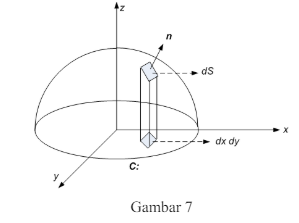
\includegraphics[width=2in]{GAMBAR 7.png}
    \end{center}
    Dengan teorema Stokes, Perhatikan separuh permukaan bola pada gambar 7.

Batas $C$ dari $S$ adalah suatu lingkaran dengan persamaan $x^2 + y^2 = 1$, $z = 0$ dan persamaan parameternya adalah $\mathbf{r} = \cos t \, \mathbf{i} + \sin t \, \mathbf{j}$, $0 \leq t \leq 2\pi$. Berdasarkan teorema Stokes $\iint_S (\nabla \times \mathbf{A}) \cdot d\mathbf{S} = \oint_C \mathbf{A} \cdot d\mathbf{r}$.
\end{frame}

\begin{frame}
\[
\begin{aligned}
\mathbf{A} \cdot d\mathbf{r} &= [(2x - y)\mathbf{i} + yz^2\mathbf{j} - y^2z\mathbf{k}] \cdot (dx \mathbf{i} + dy \mathbf{j} + dz \mathbf{k}) \\
&= (2\cos t - \sin t) (-\sin t \, dt) + 0 + 0 \\
&= -2 \sin t \cos t + \sin^2 t \, dt \\
&= \int_0^{2\pi} (-2 \sin t \cos t + \sin^2 t) \, dt \\
&= \int_0^{2\pi} \left( \frac{- \sin 2t}{2} + \frac{1 - \cos 2t}{2} \right) dt \\
&= \left[ \frac{\cos 2t}{2} + \frac{t}{2} - \frac{\sin 2t}{4} \right]_0^{2\pi} = \pi
\end{aligned}
\]
\end{frame}
\end{document}